\documentclass[conference]{IEEEtran}
\IEEEoverridecommandlockouts
\usepackage{amsmath,amssymb}
\usepackage{graphicx}
\usepackage{booktabs}
\usepackage{tikz}
\usetikzlibrary{arrows.meta,positioning,shapes.geometric}
\usepackage{pgfplots}
\usepgfplotslibrary{fillbetween}
\pgfplotsset{compat=1.16}
\usepackage{cite}
\usepackage[hidelinks]{hyperref}
\usepackage{microtype}

\begin{document}

\title{AI4BRAIN: An Uncertainty-Aware, Non-Clinical Cognitive Growth Agent\\with Faithful Explanations and a Measurable Human--AI Collaboration Score}

\author{\IEEEauthorblockN{Team AI4BRAIN}
\IEEEauthorblockA{CISTAC 1.0 Challenge, IEEE Computational Intelligence Society Tunisia Chapter\\
Source code: \url{https://github.com/aziz3r/ai4brain}}}

\maketitle

\begin{abstract}
We present AI4BRAIN, a learning-support agent that estimates five functional cognitive skills (memory, focus, flexibility, speed, reasoning) from five one-minute interactive tasks, tracks each skill as a Gaussian belief with explicit uncertainty, and recommends the next exercise with a plain-language justification. The design is non-clinical by construction: no diagnostic vocabulary, no population norms, no biometric sensing. A Kalman-type Bayesian update accounts for task difficulty, speed--accuracy trade-off, practice effects and attention lapses, and a widening projection cone shows where a skill might go with practice. Recommendations are chosen by a deterministic policy and only \emph{verbalised} by a language model, so the explanation is faithful to the real cause. We also define an operational AI Collaboration Score (0--100) from interaction logs. In a seeded simulation of 200 users $\times$ 5 skills $\times$ 12 sessions with a deliberately misspecified generator, the 95\% intervals cover the true ability in 97\% of cases, the posterior standard deviation falls from 25 to about 4 points, and robust damping reduces the error by 27\% under lapses. These figures come from simulation, not from human participants; a user study is the next step.
\end{abstract}

\begin{IEEEkeywords}
cognitive assessment, Bayesian filtering, uncertainty quantification, explainable AI, human--AI collaboration, privacy by design
\end{IEEEkeywords}

\section{Introduction}
Brain-training applications typically return a single score per game. Such a score hides measurement error, invites over-interpretation (``my brain is a 72''), and rarely says why a given exercise is proposed. For a learner, the useful questions are different: \emph{what can I do well, how sure are we, what should I practise next, and why?} Answering them responsibly requires three commitments that the CISTAC 1.0 brief makes explicit: (i) no clinical diagnosis, (ii) uncertainty everywhere a capacity is reported, and (iii) a justification for each recommendation in language that a non-expert can check.

We contribute: (1) a taxonomy of five functional skills with one-minute task protocols and closed-form scores (Section~\ref{sec:tasks}); (2) a Bayesian ``Brain Twin'' that is robust to lapses and keeps uncertainty strictly positive (Section~\ref{sec:twin}); (3) a faithful-by-design coach in which a deterministic policy decides and a language model only explains, with a bilingual clinical-vocabulary guardrail (Section~\ref{sec:coach}); (4) an explicit, auditable AI Collaboration Score (Section~\ref{sec:collab}); (5) architectural privacy controls (Section~\ref{sec:privacy}); and (6) a reproducible simulation study and an honest account of what is not yet validated (Sections~\ref{sec:eval} and~\ref{sec:limits}).

\section{Background and Related Work}
\textbf{Executive functions.} Miyake et al.\ showed that updating, inhibition and shifting are separable yet correlated executive functions~\cite{miyake2000}. We adopt this functional view and add processing speed~\cite{salthouse1996} and inductive reasoning~\cite{raven1938}. Our tasks are standard paradigms: the $n$-back~\cite{kirchner1958}, the Eriksen flanker~\cite{eriksen1974}, cued task switching~\cite{monsell2003} and choice reaction time, whose mean RT grows with $\log_2$ of the number of alternatives~\cite{hick1952}.

\textbf{Psychometrics and practice effects.} Performance rises with repetition even when ability is unchanged~\cite{calamia2012}; difference scores such as switch cost are less reliable than raw scores. We therefore model early sessions as noisier and report ranges rather than points. Sensitivity indices for $n$-back use the log-linear correction for extreme rates~\cite{hautus1995}.

\textbf{Bayesian tracking.} Linear-Gaussian state-space filtering~\cite{kalman1960} gives a recursive posterior with a closed-form update, which is cheap, inspectable and easy to explain. Robustness to outliers is handled by variance inflation of the innovation, a standard heuristic related to heavy-tailed likelihoods.

\textbf{Explainability.} Explanations are most useful when they are contrastive and selective~\cite{miller2019}, and interpretability should be evaluated against its purpose~\cite{doshi2017}. We make explanations faithful by construction: the explained quantity is the one that actually drove the decision.

\textbf{Privacy.} We follow data-minimisation, storage-limitation and erasure principles of the GDPR~\cite{gdpr}.

\section{System Overview}
Figure~\ref{fig:arch} shows the architecture. A Next.js 14 client runs the five games and sends a structured session payload to a FastAPI service. The service updates the Brain Twin, logs collaboration events, runs the coach policy, and (optionally) calls a language model to verbalise the decision. All text shown to the user passes a guardrail. Data contracts are defined once as JSON Schema and generated to Pydantic v2 and TypeScript types, so client and server cannot drift.

\begin{figure}[t]
\centering
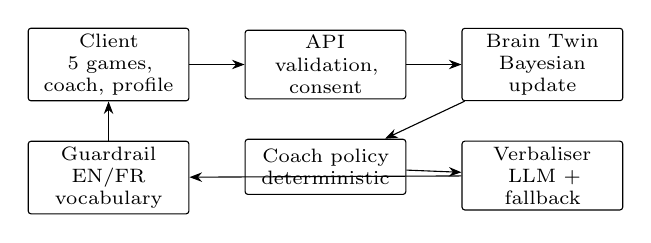
\begin{tikzpicture}[font=\scriptsize,node distance=5mm and 7mm,
 box/.style={draw,rounded corners=1pt,align=center,minimum height=7mm,inner sep=2pt,text width=1.9cm},
 arr/.style={-{Stealth[length=1.6mm]}}]
\node[box] (ui) {Client\\5 games, coach, profile};
\node[box,right=of ui] (api) {API\\validation, consent};
\node[box,right=of api] (twin) {Brain Twin\\Bayesian update};
\node[box,below=of api] (pol) {Coach policy\\deterministic};
\node[box,below=of twin] (llm) {Verbaliser\\LLM + fallback};
\node[box,below=of ui] (guard) {Guardrail\\EN/FR vocabulary};
\draw[arr] (ui)--(api); \draw[arr] (api)--(twin); \draw[arr] (twin)--(pol);
\draw[arr] (pol)--(llm); \draw[arr] (llm)--(guard); \draw[arr] (guard)--(ui);
\end{tikzpicture}
\caption{Data flow. The policy decides; the language model only explains; every string is checked before display.}
\label{fig:arch}
\end{figure}

\section{Cognitive Taxonomy and Task Protocols}\label{sec:tasks}
Each skill is assessed by one task of 36--60 trials (about 60--90 s of scored play), at one of five discrete difficulty levels $d\in\{0.5,0.75,1,1.5,2\}$ (Table~\ref{tab:tasks}). Difficulty is fixed within a session to keep the measurement clean and adapted between sessions. Each score maps to $[0,100]$ with closed forms, using $\mathrm{clip}(x)=\min(\max(x,0),1)$.

\begin{table}[t]
\caption{Skills, tasks and raw scores. $d'$: sensitivity; $I$: incongruent minus congruent RT (ms); $SC_{rel}$: relative switch cost; $\mathrm{rel}=\mathrm{median\,RT}/b_k$ with $b_k=230+130\log_2 k$; $p$: difficulty-weighted accuracy.}
\label{tab:tasks}
\centering\scriptsize
\setlength{\tabcolsep}{2pt}
\begin{tabular}{@{}p{1.15cm}p{1.45cm}p{0.9cm}p{3.6cm}@{}}
\toprule
Skill & Task & Trials & Raw score \\
\midrule
Memory & Spatial $n$-back ($n$=1--3) & 24 & $100\,\mathrm{clip}(d'/3.4)$ \\
Focus & Flanker arrows & 40 & $100\,\mathrm{clip}(1-I/250)\,\mathrm{acc}_{inc}$ \\
Flexibility & Cued switching & 36 & $100\,\mathrm{clip}(1-SC_{rel}/0.6)\,\mathrm{acc}_{sw}$ \\
Speed & Choice RT ($k$=2--6) & 60 & $100\,\mathrm{clip}\!\big(\tfrac{1.6-\mathrm{rel}}{0.9}\big)\mathrm{acc}^2$ \\
Reasoning & Matrices, 1--3 rules & 6 & $100\,\mathrm{clip}\!\big(\tfrac{p-1/6}{5/6}\big)$ \\
\bottomrule
\end{tabular}
\end{table}

Design choices follow documented biases. The $n$-back score uses $d'$ with a log-linear correction; with 8 targets and 16 non-targets its maximum is 3.48, hence the divisor 3.4. Interference and switch cost are difference scores and are normalised (switch cost by repeat RT) to limit the slow-responder bias. The matrix score is corrected for guessing (six options). Anticipations ($<$150\,ms) are dropped, and omissions count as errors. Each game is preceded by a briefing with a demonstration, and a practice round on first use, because unfamiliarity is a major source of early-session noise.

\section{The Brain Twin: Probabilistic Skill Model}\label{sec:twin}
\subsection{State and observation}
For each skill, the latent capacity $\theta\in[0,100]$ follows a random walk with drift variance $Q$, and a session yields an observation $y$:
\begin{align}
\theta_t&=\theta_{t-1}+w_t,& w_t&\sim\mathcal N(0,Q),\\
y_t&=\theta_t+v_t,& v_t&\sim\mathcal N(0,R_t).
\end{align}
The prior is $\theta\sim\mathcal N(\mu,\sigma^2)$, initialised at $(50,25)$ (maximal ignorance). We set $Q=2.5$, so uncertainty never collapses to zero, which formalises that ability changes over time.

\subsection{Observation model}
Given a raw score $s$, mean RT $\tau$, baseline RT $b$ and difficulty $d$, the observation is
\begin{equation}
y=\mathrm{clip}_{[0,100]}\!\big(s\,m + 10\log_2 d\big),\quad m=1+\mathrm{clip}\!\Big(\tfrac{b-\tau}{b}\,\tfrac{s}{100}\Big)
\end{equation}
where the speed modifier is clipped to $[-0.25,0.35]$. Weighting by $s/100$ withholds the speed bonus from fast but inaccurate responses (speed--accuracy trade-off). The logarithmic term credits the same score obtained on a harder task. For tasks whose score already contains speed (choice RT) or where speed is not the construct (matrices), $\tau=b$ is sent so that speed is not counted twice.

\subsection{Measurement noise}
\begin{equation}
R_t=\Big(10\sqrt{d}\,\big(1+\tfrac12 e^{-t/3}\big)\Big)^2 .
\end{equation}
Harder tasks and early sessions are noisier, which encodes practice and familiarisation effects as reduced trust rather than as a bias correction.

\subsection{Update with outlier damping}
With $P=\sigma^2+Q$, innovation $e=y-\mu$ and $z=|e|/\sqrt{P+R}$, a lapse ($z>3$) inflates the noise, $R\leftarrow R\,(z/3)^2$. Then
\begin{equation}
K=\frac{P}{P+R},\quad \mu'=\mu+Ke,\quad \sigma'^2=(1-K)P,
\end{equation}
and the 95\% interval is $\mu'\pm1.96\sigma'$, clipped to $[0,100]$. For constant $R$ the uncertainty converges to the fixed point $\sigma_\infty^2=\tfrac12\big(-Q+\sqrt{Q^2+4QR}\big)$. With $Q=2.5$ and $R=100$ this gives $\sigma_\infty\approx3.8$, close to the simulated floor (Fig.~\ref{fig:conv}).

\subsection{Projection cone}
The profile screen shows a projection over $k$ weeks with $\sigma_k^2=\sigma^2+4kQ$ (about four sessions per week), so the cone always widens. It is a prediction of the model under continued practice, not of an individual's outcome, and the interface says so.

\section{Faithful Explainable Coach}\label{sec:coach}
\textbf{Policy.} The next skill maximises
\begin{equation}
\pi_j=0.4\,\mathrm{clip}\!\big(\tfrac{75-\mu_j}{75}\big)+0.4\,\mathrm{clip}\!\big(\tfrac{\sigma_j}{25}\big)+0.2\,\mathrm{clip}\!\big(\tfrac{\Delta_j}{7}+0.2\big)
\end{equation}
over skills other than the last one practised, where $\Delta_j$ is days since last practice. The three terms are room to grow, value of information, and spaced coverage. The target difficulty moves towards a performance of about 70/100, in the spirit of working in the zone of proximal development: $d_{next}=\mathrm{snap}\big(d+0.5\,(s-70)/30\big)$.

\textbf{Faithfulness.} The policy returns a decision trace (task, difficulty, factors with $\mu$, $\sigma$ and a signal label). The language model receives the trace and may not change it. Its output must be a JSON object that (i) validates against the payload schema, (ii) copies the trace fields exactly, (iii) contains no number absent from the trace, and (iv) passes the guardrail; otherwise we retry twice and fall back to a template. Because the justification is generated from the quantities that determined the choice, it cannot invent a cause. Users can ask \emph{why}, receive a contrastive counterfactual, or propose another task; these actions are logged as collaboration events.

\textbf{Non-clinical guardrail.} A multilingual filter rejects diagnostic and pathological vocabulary and normative comparisons in English and French. A Monte-Carlo test runs 200 randomised traces per language and asserts zero violations and zero unauthorised numbers. Wording rules require ``estimate'', ``suggests'' and ranges, and forbid fixed-ability statements.

\section{AI Collaboration Score}\label{sec:collab}
The score is $0.20\,C+0.25\,V+0.20\,I+0.20\,A+0.15\,R$, with each component in $[0,100]$ computed from logged events:
\begin{itemize}
\item \textbf{Clarification $C$}: message informativeness (trapezoid of word count), anchoring to a result or goal, and repair of reformulations.
\item \textbf{Critical verification $V$}: weighted audit actions (asking why, challenging with a reason, modifying, accepting after reading the explanation or after a deliberate delay); blind acceptance scores 0, and indiscriminate rejection is penalised.
\item \textbf{Iteration $I$}: share of feedback followed by a revision, productive depth of exchanges, and observed score gain.
\item \textbf{Autonomy $A$}: a bell-shaped preference for consulting the coach in about 40\% of decisions, plus precision and recall of help-seeking after struggle, and retention of the final decision.
\item \textbf{Responsible use $R$}: sustainable session length, rest after fatigue signals, message rate and daily session caps, and absence of flagged content.
\end{itemize}
Each component is shrunk towards the neutral value 50, $S=50+(S_{raw}-50)\,n/(n+5)$, with standard deviation $25\sqrt{5/(n+5)}$, and the total variance is $\sum_k(w_k\sigma_k)^2$. With no data the score is 50 with a wide interval; the interface hides it until at least eight interactions and two recommendation responses are logged. The trapezoid bounds and the 40\% target are design parameters, not empirical constants.

\section{Privacy, Ethics and Non-Clinical Scope}\label{sec:privacy}
Privacy is architectural. Data are keyed by a random pseudonym; no name, e-mail, camera, microphone or keystroke dynamics are used (``non-biometric mode'' is a constant of the payload schema). Consent with a retention period (30, 90 or 365 days) is required before any assessment is accepted (HTTP 403 otherwise). Users can export all data and hard-delete it with a receipt, and a purge routine removes records whose retention period has lapsed (exposed as an endpoint; scheduling is left to deployment). The interface states that the tool is not a medical or psychological assessment, never compares a user to others, and presents scores as personal reference points on a $0$--$100$ scale. The main residual risks are misinterpretation of estimates and over-reliance on the coach, which we address with ranges, plain-language explanations and the collaboration score itself.

\section{Evaluation}\label{sec:eval}
\subsection{Simulation protocol}
We simulate 200 users $\times$ 5 skills $\times$ 12 sessions (seed 7). True ability starts at $\mathcal N(65,10^2)$ and follows a random walk with step SD 1. The observed score is $\theta_t+6e^{-s/4}+\mathcal N(0,8^2)$, clipped to $[0,100]$, with a 4\% chance of a lapse $\mathcal U(0,25)$. The generator differs from the estimator (practice bonus, noise level), so the test probes misspecification. We compare the deployed engine with damping to a variant without damping. Code: \texttt{scripts/report\_figures.py}.

\begin{figure}[t]
\centering
\begin{tikzpicture}
\begin{axis}[width=0.98\columnwidth,height=4.6cm,xlabel={session},ylabel={points},xmin=1,xmax=12,ymin=0,ymax=13,
 legend style={font=\scriptsize,at={(0.98,0.97)},anchor=north east,draw=none,fill=none},tick label style={font=\scriptsize},label style={font=\scriptsize},grid=major,grid style={gray!20}]
\addplot[thick,blue!60!black,mark=*,mark size=1pt] table[x=session,y=sigma] {data/convergence.dat};
\addlegendentry{posterior SD $\sigma$}
\addplot[thick,red!70!black,mark=square*,mark size=1pt] table[x=session,y=rmse_rob] {data/convergence.dat};
\addlegendentry{RMSE, with damping}
\addplot[thick,orange!80!black,dashed,mark=triangle*,mark size=1pt] table[x=session,y=rmse_non] {data/convergence.dat};
\addlegendentry{RMSE, no damping}
\end{axis}
\end{tikzpicture}
\caption{Posterior SD and estimation error against the true ability (simulation, 1000 trajectories). Damping lowers the error once lapses occur.}
\label{fig:conv}
\end{figure}

\subsection{Results}
Table~\ref{tab:res} summarises the simulation. The posterior SD falls from 25 (prior) to 11.9 after one session, 7.1 after three and 4.1 after twelve. The estimation error follows (RMSE 10.2 to 3.6). Coverage of the nominal 95\% interval is about 97\% for the deployed engine: slightly conservative, as expected because the estimator assumes more noise (SD 10) than the generator (8). Without damping the coverage falls to 90.6\% at session 12 and the RMSE is 4.8, a 36\% larger error: lapses bias the mean and the interval no longer reflects them. Damping detects 83\% of lapses with a 0.12\% false-damping rate. A positive bias of about 1.6 points at session 3 reflects the practice effect, which the model absorbs as noise, not as a bias correction (the bias is $<$0.2 by session 12).

\begin{table}[t]
\caption{Simulation results (200 users $\times$ 5 skills, seed 7).}
\label{tab:res}
\centering\footnotesize
\begin{tabular}{@{}lrr@{}}
\toprule
Metric & Damping & No damping\\
\midrule
RMSE vs true ability, session 12 & 3.55 & 4.84\\
95\% interval coverage, session 12 & 97.2\% & 90.6\%\\
Posterior SD, sessions 1 / 3 / 12 & \multicolumn{2}{r}{11.9 / 7.1 / 4.1}\\
Lapses damped / false damping & 82.6\% / 0.12\% & --\\
Corr.\ final estimate vs true ability & 0.94 & --\\
Corr.\ estimate at sessions 8 and 12 & 0.95 & --\\
\bottomrule
\end{tabular}
\end{table}

A worked lapse (Fig.~\ref{fig:lapse}) shows the intended behaviour: a raw score of 3 at session 7 in a stable run around 72 moves the estimate from 70.9 to 66.6 (about 4 points, with a visibly wider interval) and the profile recovers within three sessions.

\begin{figure}[t]
\centering
\begin{tikzpicture}
\begin{axis}[width=0.98\columnwidth,height=4.3cm,xlabel={session},ylabel={score},xmin=1,xmax=12,ymin=0,ymax=100,
 legend style={font=\scriptsize,at={(0.98,0.05)},anchor=south east,draw=none,fill=white,fill opacity=0.8},tick label style={font=\scriptsize},label style={font=\scriptsize},grid=major,grid style={gray!20}]
\addplot[name path=hi,draw=none] table[x=session,y=hi] {data/lapse_example.dat};
\addplot[name path=lo,draw=none] table[x=session,y=lo] {data/lapse_example.dat};
\addplot[teal!40] fill between[of=hi and lo];
\addplot[thick,teal!60!black] table[x=session,y=mu] {data/lapse_example.dat};
\addlegendentry{estimate and 95\% range}
\addplot[only marks,mark=x,red!70!black] table[x=session,y=raw] {data/lapse_example.dat};
\addlegendentry{raw score}
\end{axis}
\end{tikzpicture}
\caption{A lapse at session 7 is damped; the estimate moves about 4 points and recovers.}
\label{fig:lapse}
\end{figure}

\subsection{Software verification and interface}
The backend has 19 automated tests (engine, collaboration score, schema validation, consent gate, export and deletion, purge with a fake clock, and the language check) which pass. The interface is bilingual (English/French) with a plain editorial design; Fig.~\ref{fig:ui} shows a game briefing and the profile screen. The profile screen of the figure is populated with a seeded demonstration persona, not with measurements of a real person.

\begin{figure*}[t]
\centering
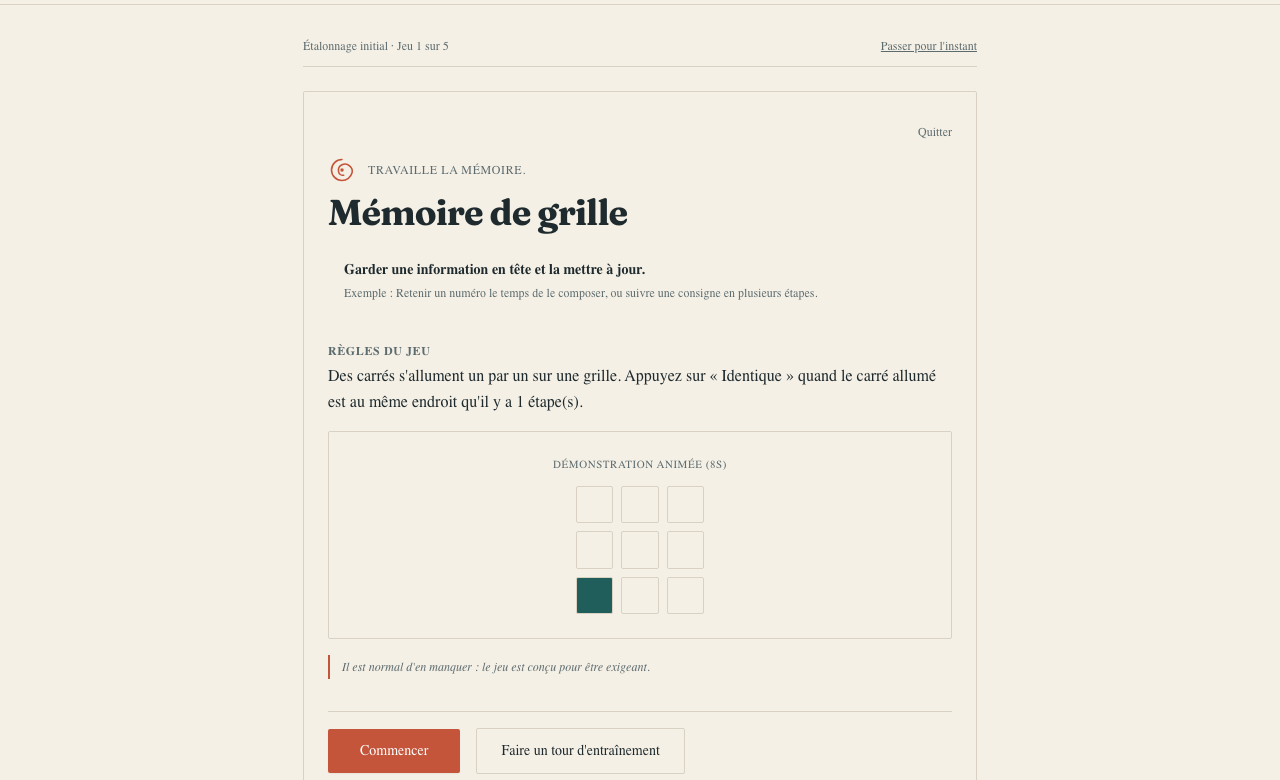
\includegraphics[width=0.485\textwidth]{fig/briefing_fr.png}\hfill
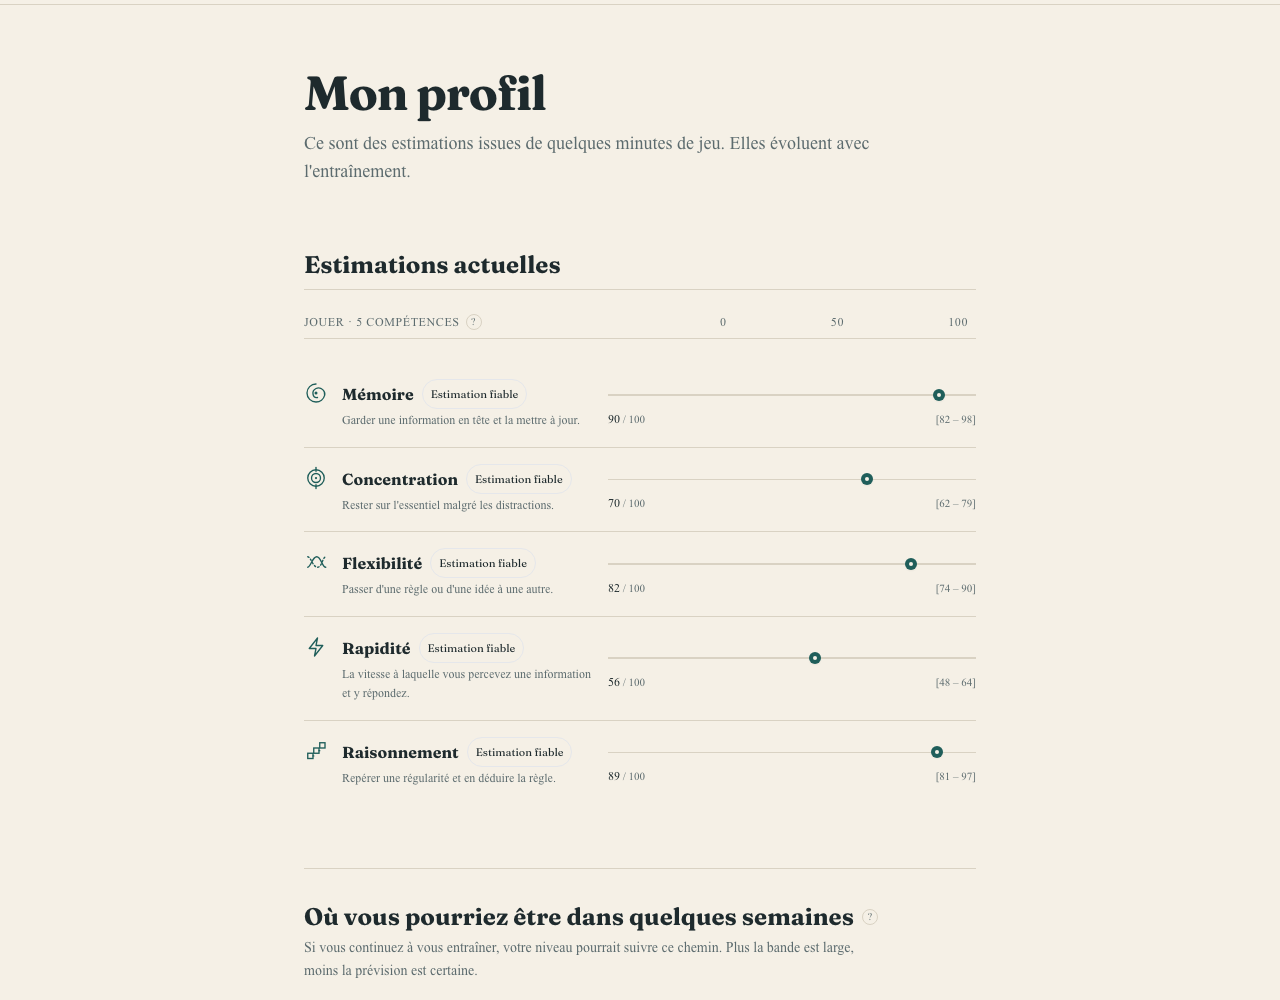
\includegraphics[width=0.485\textwidth]{fig/profile_fr.png}
\caption{Interface (French): game briefing with an animated example, and profile with one range line per skill (seeded demo persona).}
\label{fig:ui}
\end{figure*}

\section{Limitations and Future Work}\label{sec:limits}
\textbf{No human validation yet.} All reliability and coverage figures are from simulation with a known generator; they show that the estimator behaves as designed under misspecification, not that it measures people validly. Test--retest reliability, convergent validity with established tasks, and the real distribution of scores at the coach's chosen difficulty must be measured with participants. A usability study with non-expert users has been specified but has not been run, so we make no usability claim.
\par\textbf{Short tasks.} One minute of play gives noisy estimates, especially for reasoning (six items) and difference scores; the ranges are wide on purpose. Per-skill noise scales are a planned refinement.
\par\textbf{Model simplicity.} Skills are modelled independently with Gaussian noise; correlations between skills, learning-curve models, and non-Gaussian likelihoods could sharpen estimates.
\par\textbf{Constants.} The weights of the policy, the collaboration-score trapezoids and the speed coefficients are design parameters that need calibration.
\par\textbf{Language model.} Faithfulness covers the decision and numbers; the tone of free text depends on the model, which is why every output is validated and a template fallback exists.
\par\textbf{Security.} The prototype has no user authentication: the random pseudonym acts as a bearer secret for export and deletion. The purge endpoint requires an administrator token, disabled unless one is configured. A deployment would add authenticated sessions.
\par\par\textbf{Interface.} The bilingual interface was checked by an automated pass over every route in both languages; it was not reviewed by native-speaking users.

\section{Conclusion}
AI4BRAIN shows that a learning-support agent can be honest about uncertainty, explain itself faithfully, remain strictly non-clinical, and quantify how well a user works with its advice, using small, inspectable models. The next milestone is an empirical study that turns simulated reliability into measured reliability.

\section*{Acknowledgment}
We thank the CISTAC 1.0 organisers. Generative AI tools were used to assist with drafting text and code; the authors reviewed all content and are responsible for it.

\begin{thebibliography}{99}
\bibitem{miyake2000} A.~Miyake \emph{et~al.}, ``The unity and diversity of executive functions and their contributions to complex frontal lobe tasks: A latent variable analysis,'' \emph{Cognitive Psychology}, vol.~41, no.~1, pp.~49--100, 2000.
\bibitem{salthouse1996} T.~A. Salthouse, ``The processing-speed theory of adult age differences in cognition,'' \emph{Psychological Review}, vol.~103, no.~3, pp.~403--428, 1996.
\bibitem{raven1938} J.~C. Raven, \emph{Progressive Matrices: A Perceptual Test of Intelligence}. London: H.~K. Lewis, 1938.
\bibitem{kirchner1958} W.~K. Kirchner, ``Age differences in short-term retention of rapidly changing information,'' \emph{J. Experimental Psychology}, vol.~55, no.~4, pp.~352--358, 1958.
\bibitem{eriksen1974} B.~A. Eriksen and C.~W. Eriksen, ``Effects of noise letters upon the identification of a target letter in a nonsearch task,'' \emph{Perception \& Psychophysics}, vol.~16, no.~1, pp.~143--149, 1974.
\bibitem{monsell2003} S.~Monsell, ``Task switching,'' \emph{Trends in Cognitive Sciences}, vol.~7, no.~3, pp.~134--140, 2003.
\bibitem{hick1952} W.~E. Hick, ``On the rate of gain of information,'' \emph{Quarterly J. Experimental Psychology}, vol.~4, no.~1, pp.~11--26, 1952.
\bibitem{calamia2012} M.~Calamia, K.~Markon, and D.~Tranel, ``Scoring higher the second time around: Meta-analyses of practice effects in neuropsychological assessment,'' \emph{The Clinical Neuropsychologist}, vol.~26, no.~4, pp.~543--570, 2012.
\bibitem{hautus1995} M.~J. Hautus, ``Corrections for extreme proportions and their biasing effects on estimated values of $d'$,'' \emph{Behavior Research Methods, Instruments, \& Computers}, vol.~27, no.~1, pp.~46--51, 1995.
\bibitem{kalman1960} R.~E. Kalman, ``A new approach to linear filtering and prediction problems,'' \emph{J. Basic Engineering}, vol.~82, no.~1, pp.~35--45, 1960.
\bibitem{miller2019} T.~Miller, ``Explanation in artificial intelligence: Insights from the social sciences,'' \emph{Artificial Intelligence}, vol.~267, pp.~1--38, 2019.
\bibitem{doshi2017} F.~Doshi-Velez and B.~Kim, ``Towards a rigorous science of interpretable machine learning,'' arXiv:1702.08608, 2017.
\bibitem{gdpr} European Parliament and Council, ``Regulation (EU) 2016/679 (General Data Protection Regulation),'' 2016.
\end{thebibliography}
\end{document}
